\documentclass[border=4pt]{standalone}
\usepackage{pgfplots}
\pgfplotsset{compat=1.18}

\begin{document}
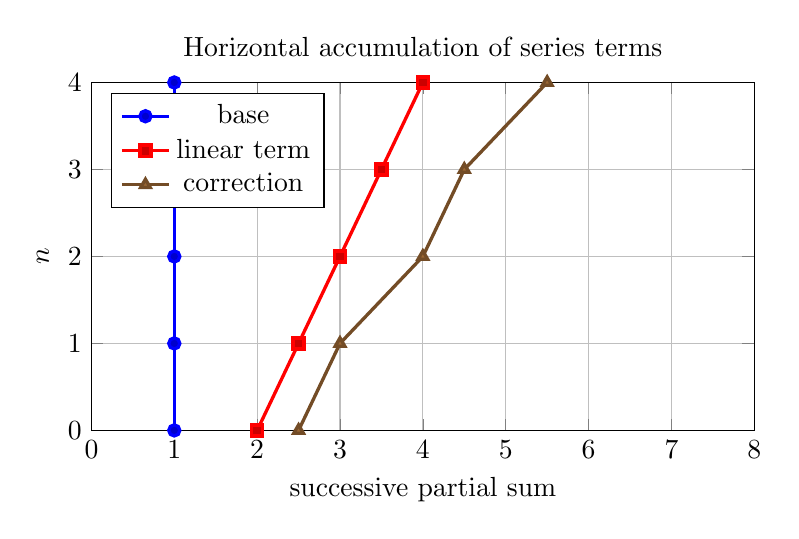
\begin{tikzpicture}
  \begin{axis}[
    stack plots=x,
    width=10cm,
    height=6cm,
    xmin=0,
    xmax=8,
    ymin=0,
    ymax=4,
    xlabel={successive partial sum},
    ylabel={$n$},
    title={Horizontal accumulation of series terms},
    grid=major,
    legend pos=north west
  ]
    \addplot+[very thick,mark=*] coordinates {(1,0) (1,1) (1,2) (1,3) (1,4)};
    \addplot+[very thick,mark=square*] coordinates {(1,0) (1.5,1) (2,2) (2.5,3) (3,4)};
    \addplot+[very thick,mark=triangle*] coordinates {(0.5,0) (0.5,1) (1,2) (1,3) (1.5,4)};
    \legend{base,linear term,correction}
  \end{axis}
\end{tikzpicture}
\end{document}
